\section{Monday for MAT4002}\index{Monday_lecture}

\subsection{Isomorphsim between Edge Loop Group and the Fundamental Group}

Recall that 
\[
\pi_1(X,b):=\{[\ell]\mid \ell:[0,1]\to X\text{ denotes the loops based at $b$}\}
\]
and 
\[
E(K,b)=\{[\alpha]\mid \alpha\text{ is an edge loop in $K$ based at $b$}\}
\]
Now we show that the mapping defined below is injective:
\[
\begin{array}{ll}
\theta:&E(K,b)\to\pi_1(|K|,b)\\
\text{with}&[\alpha]\mapsto[|g_\alpha|]
\end{array}
\]
\begin{itemize}
\item
Let $\alpha=(v_0,\dots,v_n)$ be an edge loop based at $b$ such that $\theta([\alpha])=e$, i.e., 
$|g_\alpha|\simeq c_b$.
It suffices to show that $[\alpha]$ is the identity element of $E(K,b)$.
\item
Choose a homotopy $H:|g_\alpha|\simeq c_b$ such that $H:I\times I\to|K|$.
The graphic illustration for $H$ is shown in Fig.~(\ref{fig:13:1}).
\begin{figure}[H]
\centering
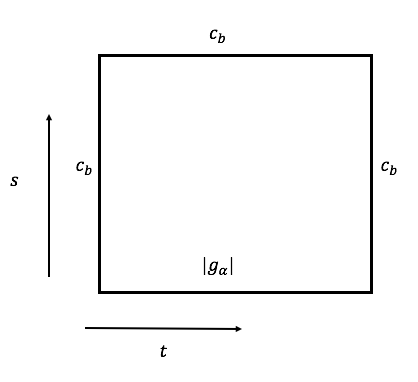
\includegraphics[width=0.5\textwidth]{week13/f_24}
\caption{Graphic illustration for $H:I\times I\to|K|$}
\label{fig:13:1}
\end{figure}
Now apply the simplicial approximation theorem, there exists a subdivision of $I\times I$, denoted as $(I\times I)_{(r)}$~(for sufficiently large $r$), shown in the Fig.~(\ref{fig:13:2})
\begin{figure}[H]
\centering
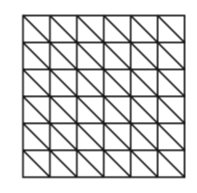
\includegraphics[width=0.4\textwidth]{week13/f_25}
\caption{Graphic illustration for $(I\times I)_{(r)}$.
In particular, divide $I\times I$ into $r^2$ congruent squares, and then further divide each of these squares along the diagonal to form $(I\times I)_{(r)}$.} 
\label{fig:13:2}
\end{figure}
such that $|(I\times I)_{(r)}|=I\times I$, and there exists the simplicial map
\[
\begin{array}{ll}
G:&(I\times I)_{(r)}\to K\\
\text{such that}&|G|\simeq H.
\end{array}
\]
Without loss of generality, assume $r$ is a sufficiently large multiple of $n$.

The graphic illustration of $|G|$ is shown in Fig.~(\ref{fig:13:3}):
\begin{figure}[H]
\centering
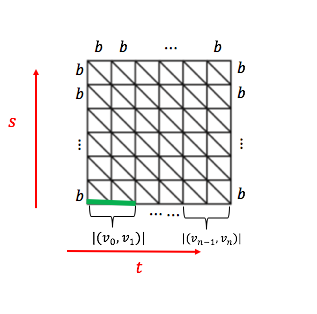
\includegraphics[width=0.4\textwidth]{week13/f_26}
\caption{Graphic illustration for the mapping $|G|$.
} 
\label{fig:13:3}
\end{figure}
In particular, $|G|$ maps $\{0,1\}\times I$ into $\{b\}$; $I\times\{1\}$ into $\{b\}$; 
$(i/n,0)$ into $\{v_i\}, i=0,\dots,n$, and $[i/n,(i+1)/n]$ into $|(v_i,v_{i+1})|, i=0,\dots,n-1$.
\item
Consider the simplicial subcomplex of $(I\times I)_{(r)}$ shown in Fig.~(\ref{fig:13:4})
\begin{figure}[H]
\centering
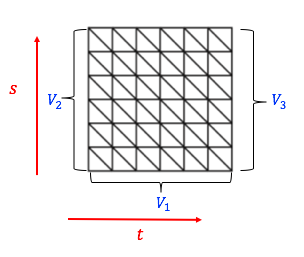
\includegraphics[width=0.4\textwidth]{week13/f_27}
\caption{Graphic illustration for the simplicial subcomplex $V_1,V_2,V_3$.
} 
\label{fig:13:4}
\end{figure}
For instance, $V_1$ has $(r+1)$ $0$-simplicies and $r$ 1-simplies. It follows that
\[
H(|V_1|)=H(|V_2|)=H(|V_3|)=\{b\}.
\]
By proposition~(\ref{pro:10:6}), we can pick $G$ be such that 
\[
G(V_1)=G(V_2)=G(V_3)=\{b\}.
\]
Consider $W_1$ as the simplicial subcomplex of $(I\times I)_{(r)}$ given by the green line shown in Fig.~(\ref{fig:13:3}), which follows that 
\[
H(|W_1|) = \{v_0,v_1\}
\implies G(W_1)=\{v_0,v_1\}
\]

Similarly, 
\[
H(|W_i|)=\{v_{i-1},v_i\}\implies
G(W_i)=\{v_{i-1},v_i\}, \forall 1\le i\le n.
\]
As a result, $|G|(|V_1|)=\beta:=(bv_0\cdots v_0v_1\cdots v_1\cdots v_n\cdots v_nb)$, and clearly,
\begin{align*}
\beta&\sim(bv_0v_1v_2\cdots v_{n-1}v_nb)\\
&\sim(bv_1v_2\cdots v_{n-1}b)=\alpha
\end{align*}
\item
Now it suffices to show $\beta\simeq e$. This is true by the sequence of elementary contractions and expansions as shown in the Fig.~(\ref{fig:13:5}).
\begin{figure}[H]
\centering
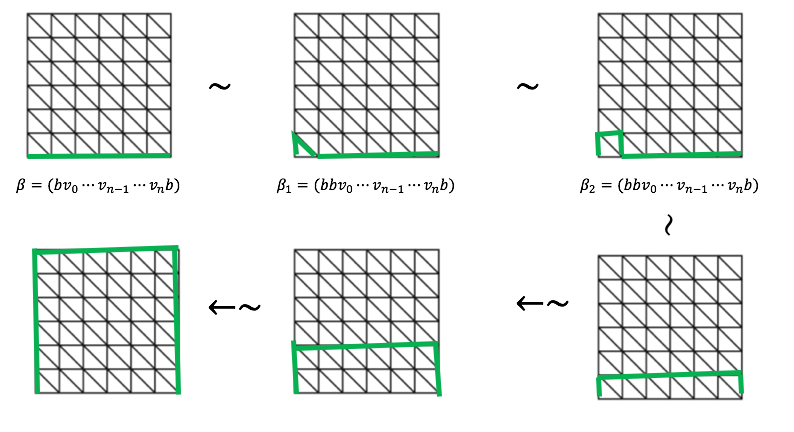
\includegraphics[width=\textwidth]{week13/f_28}
\caption{A sequence of elementary contractions and expansions to show that $\beta\sim(b\cdots b)=(b)$.
} 
\label{fig:13:5}
\end{figure}


\end{itemize}




\begin{remark}
The definition of $E(K,b)$ only involves $n$-simplicials for $n\le 2$.
\end{remark}

\begin{proposition}
For any simplicial complex $K$, consider the simplicial subcomplex $\text{Skel}^n(K)=(V_k,\Sigma_K^n)$, 
where $\Sigma_K^n$ consists of $\sigma\in\Sigma_K$ with $|\sigma|\le n+1$ (this is the $n$-skeleton of $K$).
Then 
\[
\pi_1(|K|,b)\cong\pi_1(|\text{Skel}^2(K)|,b)
\]
\end{proposition}

\begin{proof}
Since $E(K,b)$ only involves $n$-simplicials for $n\le 2$, we imply $E(K,b)\cong E(\text{Skel}^2(K),b)$.

Moreover, $\pi_1(|K|,b)\cong E(K,b)$ and $\pi_1(|\text{Skel}^2(K)|,b)\cong E(\text{Skel}^2(K),b)$.

The proof is complete.
\end{proof}




\begin{corollary}\label{cor:13:2}
For $n\ge 2$, $\pi_1(S^n)$ is a trivial fundamental group.
\end{corollary}

\begin{proof}
Consider the simplicial complex $K$ with
\[
\begin{array}{ll}
V=\{1,2,\dots,n+2\},
&
\Sigma=\{\text{all proper subsets of $V$}\}
\end{array}
\]
It's clear that $|K|\cong S^n$, and $\text{Skel}^2(K)$ has
\begin{itemize}
\item
$V:\{1,\dots,n+2\}$
\item
$\Sigma^2:$ all subsets of $V$ with less or equal to $3$ elements.
\end{itemize}
For any edge loop $a$ in $\pi_1(|\text{skel}^2(K)|)$, we have
\begin{align*}
a&=(bv_0v_1v_2\cdots v_n)\\
&\sim(bv_1v_2\cdots v_{n-2}v_{n-1}b)\\
&\sim\cdots\\
&\sim(b)
\end{align*}
Therefore, all edge loops $\alpha$ in $\pi_1(|\text{skel}^2(K)|)$ satisfies $[\alpha]=[(b)]=e$., i.e.,
\[
\pi_1(|\text{skel}^2(K)|)\cong\{e\},
\]
which implies $\pi_1(|K|) \cong\pi_1(|\text{skel}^2(K)|)\cong\{e\}$.
Since $|K|\cong S^n$, we imply 
\[
\pi_1(S^n)\cong \pi_1(|K|) \cong\{e\}.
\]
\end{proof}
\begin{remark}
The Corollary~(\ref{cor:13:2}) does not hold for $S^1$ since the constructed $\Sigma^2$ for $S^1$ 
does not contain $\{1,2,3\}.$
\end{remark}

\begin{theorem}
$\pi_1(S^1)\cong\mathbb{Z}$.
\end{theorem}
\begin{proof}
Construct the triangle $K$ shown in Fig.~(\ref{fig:13:6}), and it's clear that $|K|\cong S^1$.
\begin{figure}[H]
\centering
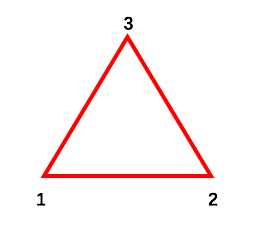
\includegraphics[width=0.3\textwidth]{week13/f_29}
\caption{Triangle $K$ such that $|K|\cong S^1$
} 
\label{fig:13:6}
\end{figure}
It suffices to show $E(K,1)\cong\mathbb{Z}$.
Define the orientation of $|K|$ as shown in Fig.~(\ref{fig:13:7}).
\begin{figure}[H]
\centering
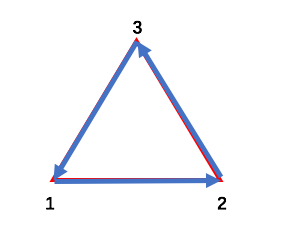
\includegraphics[width=0.3\textwidth]{week13/f_30}
\caption{Orientation of $|K|$
} 
\label{fig:13:7}
\end{figure}
Any edge loop $\alpha$ based at $1$ is equivalent to the canonical form
\[
\alpha\sim(1bc1bc\cdots 1bc1),\quad
\text{where $bc=32$ or $23$.}
\]

We construct the isomorphism between $E(K,b)$ and $\mathbb{Z}$ directly:
\[
\begin{array}{ll}
\phi:&E(K,b)\to\mathbb{Z}\\
\text{with}&[\alpha]\mapsto\text{winding number of $\alpha$}
\end{array}
\]
where the winding number of $\alpha$ is the number of times it traverses $(2,3)$ in the forwards direction minus the number of times it traverses $(3,2)$ in the backwards direction.

The difficult part is to show the well-definedness of $\phi$, which can be done by using canonical form of $\alpha$.
\end{proof}













